\documentclass[tikz, border = 2pt]{standalone}

%---------------------------------------------------------------------------%
% PACKAGES                                                                  %
%---------------------------------------------------------------------------%

%----- MATH
%---------------------------------------------------------------------------%
\usepackage{amsmath, amssymb}

%----- FIGURES
%---------------------------------------------------------------------------%
\usepackage{color}
\usepackage{pgfplots}
\pgfplotsset{compat=1.13}

%---------------------------------------------------------------------------%
%                                MINES COLORS                               %
%---------------------------------------------------------------------------%

%---------- OFFICIAL COLORS
\definecolor{MPTblue}{RGB}{0,94,158}

\begin{document}

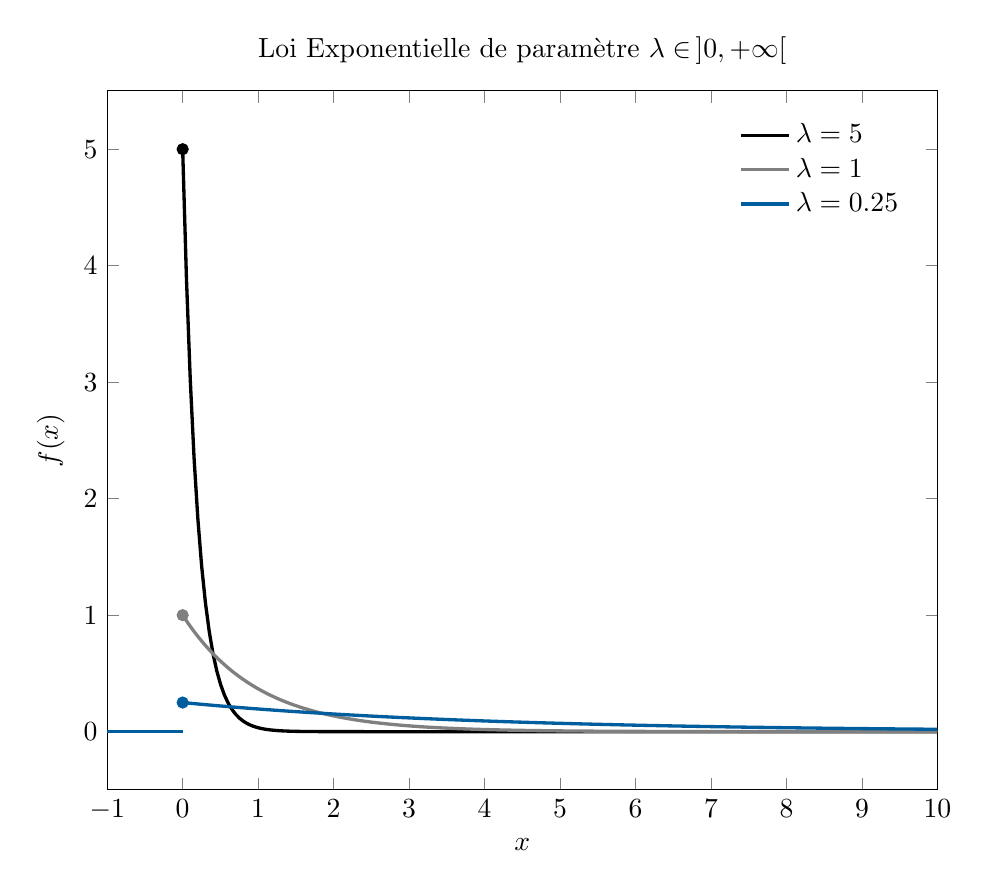
\begin{tikzpicture}
\begin{axis}[width = \textwidth,
title style = {align = center},
title={Loi Exponentielle de param\`etre $\lambda \in\, ]0,+\infty[$},
xlabel={$x$},
ylabel={$f(x)$},
legend pos = north east,
legend style = {draw=none},
legend cell align = left,
xmin = -1,
xmax = 10,
ylabel near ticks,
domain = 0:10
]
\addplot[black, very thick, samples = 2, forget plot, domain = -1:0] {0};
\addplot[black, only marks, forget plot] coordinates {(0,5)};
\addplot[black, very thick, samples = 200] {(5*exp(-5*x))*(x>=0)};
%
\addplot[black!50, very thick, samples = 2, forget plot, domain = -1:0] {0};
\addplot[black!50, only marks, forget plot] coordinates {(0,1)};
\addplot[black!50, very thick, samples = 200] {(exp(-x))*(x>=0)};
%
\addplot[MPTblue, very thick, samples = 2, forget plot, domain = -1:0] {0};
\addplot[MPTblue, only marks, forget plot] coordinates {(0,0.25)};
\addplot[MPTblue, very thick, samples = 200] {(0.25*exp(-x/4))*(x>=0)};
%
\legend{{$\lambda = 5$},{$\lambda = 1$},{$\lambda = 0.25$}}
\end{axis}
\end{tikzpicture}

\end{document}